\documentclass[inzynier,druk]{dyplom}
\usepackage[utf8]{inputenc}
\usepackage{hyperref}
\usepackage{booktabs}
%%
\usepackage[toc]{appendix}
\renewcommand{\appendixtocname}{Dodatki}
\renewcommand{\appendixpagename}{Dodatki}

% pakiet do sk?adu listing?w w razie potrzeby mo?na odblokowa? mo?liwo?? numerowania linii lub zmieni? wielko?? czcionki w listingu
\usepackage{minted}
\setminted{breaklines,
frame=lines,
framesep=5mm,
baselinestretch=1.1,
fontsize=\small,
%linenos
}

% nowe otoczenie do składania listingów
\usepackage{float}
\newfloat{listing}{htp}{lop}
\floatname{listing}{Listing}
\usepackage{chngcntr}
\counterwithin{listing}{chapter}

% patch wyr?wnuj?cy spis listing?w do lewego marginesu 
%https://tex.stackexchange.com/questions/58469/why-are-listof-and-listoffigures-styled-differently
\makeatletter
\renewcommand*{\listof}[2]{%
  \@ifundefined{ext@#1}{\float@error{#1}}{%
  \expandafter\let\csname l@#1\endcsname \l@figure% <- use layout of figure
    \float@listhead{#2}%
    \begingroup
      \setlength\parskip{0pt plus 1pt}%               % <- or drop this line completely
        \@starttoc{\@nameuse{ext@#1}}%
    \endgroup}}
\makeatother

\usepackage{url}
\usepackage{lipsum}

% Dane o pracy
\author{Karol Kowalski}
\title{Aplikacja wspomagająca zdalne szacowanie historyjek użytkownika metodą Planistycznego Pokera.}
\titlen{Aplikacja wspomagaj?ca zdalne szacowanie historyjek u?ytkownika metod? Planistycznego Pokera.}
\promotor{dr. \ hab. \ inż. \ prof. PWr. Trawiński Bogdan}
%\konsultant{dr hab. in?. Kazimerz Kabacki}
\wydzial{Wydział Informatyki i Zarządzania}
\kierunek{Informatyka}
\krotkiestreszczenie{W pracy przedstawiono projekt aplikacji umożliwiającej przeprowadzenie rozgrywki planning pokera online z użyciem ReactJS oraz Firebase.}
\slowakluczowe{Firebase, ReactJS, FLUX, planning poker, estymacja}

\begin{document}

\maketitle

\tableofcontents

\listoffigures

\listof{listing}{Spis listingów}

\listoftables

% --- Strona ze streszczeniem i abstraktem ------------------------------------------------------------------
\chapter*{Streszczenie} % po polsku
Celem pracy było opracowanie aplikacji zaprojektowanej do gry w planning pokera zdalnie. Dostępne aplikacje spełniają swoje zadanie, jednak autor nie znalazł aplikacji, która byłaby silnie zintegrowana z Github'em. Dlatego wyróżniającą cechą jego aplikacji będzie możliwość importu historyjek z Github'a które są tam w postaci issues oraz exportu ocen do Github'a w postaci etykiet. W ramach pracy autor stworzył aplikację opartą o architekturę FLUX z bazą danych firebase jako backend. Dzięki temu rozwiązaniu planning poker może być rozgrywany w czasie rzeczywistym. Oprócz tego praca zawiera omówienie pewnych metod zarządzania zwinnego. Użyteczność aplikacji będzie sprawdzona w oparciu o wyniki ankiety, które zostaną zawarte w niniejszej pracy. 


% Kilka sztuczek, ?eby:
% - Abstract pojawi? si? na tej samej stronie co Streszczenie
% - Abstract nie pojawi? si? w spisie tre?ci
\addtocontents{toc}{\protect\setcounter{tocdepth}{-1}}
\begingroup
\renewcommand{\cleardoublepage}{}
\renewcommand{\clearpage}{}
\chapter*{Abstract} % ...i to samo po angielsku
The main goal of this thesis was development of web app designed to play planing poker online. Avaliable aplications fulfil their role but however author haven't found application, which would be strongly integrated with Github. That's why distinctive feature of author's app will be possibility is importing user stories from Github projects which are there in the shape of issues and exporting story points to Github in form of labels. Within work author made aplication based on FLUX architecture with firebase database as backend. Thanks this solution planning poker can be played in real time. Except of app description thesis describe some of agile managment and estimating methods. Usability of application will be tested thanks usability survey which reasults are consist within thesis.
\endgroup
\addtocontents{toc}{\protect\setcounter{tocdepth}{2}}
% --- Koniec strony ze streszczeniem i abstraktem -----------------------------------------------------------



% Rozdzia? do??czony z zewn?trz
\chapter*{Wstęp}
Planowanie to odpowiadanie na pytanie „Co powinniśmy stworzyć i kiedy?”.
Jednak aby odpowiedzieć na to pytanie powinniśmy zadać również pytania o estymację
(„Jak duże to jest?”) oraz harmonogram („Kiedy będzie skończone\text{?}” oraz „Ile będzie zrobione do tego czasu?”).
Estymowanie i planowanie są bardzo istotne w sukcesie każdego projektu,
gdyż plany pomagają inwestorom podejmować decyzje.\cite{Cohen_2006}
\section*{Opis problemu}

W dzisiejszym świecie coraz więcej projektów jest tworzonych przez zespoły rozproszone.
Zespół rozproszony to taki, którego członkowie realizują jeden projekt,
cel i zadania w określonym czasie, pracując z różnych miejsc. 
Zespoły rozproszone pracują jak tradycyjne zespoły zadaniowe,
ale mają ze sobą na co dzień kontakt wirtualny i widują się sporadycznie.\cite{www_rozproszony}
Przez co mają problem ze spotkaniami na żywo.
Dlatego muszą się spotkać w wirtualnym pokoju a wnioski ze spotkania powinny być zapisane w centralnym miejscu projektu.
Bardzo często tym miejscem jest np. GitHub.\footnote{GitHub – hostingowy serwis internetowy przeznaczony dla projektów programistycznych wykorzystujących system kontroli wersji Git.}

\section*{Cel pracy}

Zadaniem jakie postawiłem przed sobą jest stworzenie aplikacji umożliwiającej rozegranie planning pokera w czasie rzeczywistym w raz z rolami product ownera,
scrum mastera oraz gracza by jak najwierniej zasymulować rozgrywkę w planning pokera.
Dodatkowym celem jest synchronizowanie wyników rozgrywki z aplikacją GitHub.

\section*{Zakres pracy}

Praca obejmuje opracowanie projektu aplikacji, implementację w frameworku ReactJS.\footnote{ReactJS – biblioteka języka programowania JavaScript, która wykorzystywana jest do tworzenia interfejsów graficznych aplikacji internetowych.}
oraz wdrożenie powyższego w bazie danych Firebase, a także zhostowanie tego wszystkiego na hostingu Firebase.\footnote{Firebase – to platforma do opracowywania aplikacji mobilnych i internetowych opracowana przez firmę Firebase, Inc. w 2011 roku, a następnie nabyta przez Google w 2014 roku.}
Dodatkowym zadaniem jest sprawdzenie użyteczności programu za pomocą ankiety.


% !TeX program = latexmk
% !TeX spellcheck = pl_PL
% !TeX root = example.tex

\chapter{Wprowadzenie}

Najpopularniejszą definicją projektu jest definicja Project Management Institute (PMI – międzynarodowe stowarzyszenie zrzeszające kierowników projektów.
Project Management Institute powstał w 1969 w Pensylwanii w USA jako stowarzyszenie non profit zrzeszające profesjonalistów
w dziedzinie zarządzania projektami- istnieje również oddział we Wrocławiu.): 
\begin{quote}
Projekt, to tymczasowa działalność podejmowana w celu wytworzenia unikatowego wyrobu,
dostarczenia unikatowej usługi lub otrzymania unikatowego rezultatu
\end{quote}
~\cite{PMI_2000}
Już w starożytnym Egipcie istniały metody zarządzania skomplikowanym przedsięwzięciem,
np budowa piramid. Było to olbrzymie wyzwanie, które wymagało wiedzy zarówno planistycznej,
jak i logistycznej. W ubiegłym stuleciu, w latach 50 stosowano podejścia zwane obecnie współczesnymi
technikami zarządzania projektami. Weźmy np projekt systemu rakiet balistycznych Polaris.
Okazał się on swoistym koszmarem technicznym i administracyjnym. Nad projektem pracowała olbrzymia ilość zespołów badawczych,
projektowych i produkcyjnych. Dla udokumentowania wszystkich działań zużyto tony papieru, a samo zarządzanie projektami zaczęto
uznawać za dziedzinę bardzo skomplikowaną, niedostępną, opartą na wiedzy specjalistów.\cite{Stanley_2013}

\section{Najpopularniejsze metody zarządzania projektami}
Przy dokonywaniu wyboru metodyki zarządzania projektem należy przeprowadzić adekwatną analizę w celu doboru odpowiedniego podejścia,
gdyż każda z metodyk posiada wady i zalety. Wyróżniamy dwa podejścia (klasyczne i zwinne), które różnią się dość mocno między sobą w kilku płaszczyznach (przekrojach),takich jak:
odpowiedzialność za produkt, rola menedżera w zespole, istota prac wstępnych, zdefiniowanie produktu czy odpowiedź zwrotna użytkowników.
Co uwzględniono w tabeli \~ref{tabela:roznice}.

% Tabela. Nazwa tabeli u góry.
\begin{table}
\centering\caption{ Różnice między podejściem klasycznym a zwinnym\label{tabela:roznice}}
\begin{tabular}{ p{0.25\textwidth} p{0.3\textwidth}  p{0.3\textwidth} }% wyrównanie kolumn tabeli -> l c r - do lewej, środka, do prawej
\toprule
\textbf{Płaszczyzna} &\textbf{ Podejście klasyczne} & \textbf{Podejście zwinne} \\
\midrule
\textbf{Odpowiedzialność
za produkt}
 & Podzielona między marketera,
 menadżera produktu i menadżera projektu & Istnieje tylko jeden właściciel produktu \\
\midrule
\textbf{Rola menedżera
w zespole} & oddzielony od zespołów deweloperskich & Jest członkiem zespołu i ściśle z nim współpracuje.\\
\midrule
\textbf{Istota prac wstępnych} & Przeprowadzane są szczegółowe badania rynku, planowanie produktu i analizy biznesowe
& Ograniczają się do stworzenia wizji, która ogólnie opisuje wygląd i działanie produktu. \\
\midrule
\textbf{Zdefiniowanie
produktu} & Wymagania są określane i zatwierdzane w początkowej fazie
& Produkt odkrywany jest stopniowo, a wymagania krystalizują się w trakcie
\\
\midrule
\textbf{Odpowiedź zwrotna} & Dostępna po wypuszczeniu produktu na rynek
& Wczesna i częsta odpowiedź zwrotna po małych wdrożeniach
\\
\bottomrule
\end{tabular}
\end{table}
\newpage

\section{Podejście klasyczne}

Podejście klasyczne, reprezentowane przez PMBoK (Kompendium wiedzy o zarządzaniu projektami) lub metodykę PRINCE
(kompleksowa metodą zarządzania projektami, zalicza się ją do podejścia klasycznego) oraz jej następcę PRINCE2,
ma na celu wytworzenie kompletnego produktu przy uprzednim, dokładnym określeniu jego cech.
Takie podejście charakteryzuje się ogromnym formalizmem, weźmy na przykład dokonywanie zmian,
które wiąże się z wypełnianiem dokumentów (RfC – ang. Request for Change) -prośby o zmianę.
Każda odpowiedź, to z kolei oczekiwanie, aż zostanie przeanalizowana i zatwierdzona bądź odrzucona.
Dodatkowo osoby odpowiedzialne zwykle nie pracują wraz z zespołem, w związku z czym często występują bariery komunikacyjne.\cite{www_tradycyjne_projekty}

\section{Podejście zwinne}

Podejście zwinne ukierunkowane jest na zespół, który w pełni odpowiada za wykonanie swojej części
zadania i stopniowo dostosowuje je do potrzeb przyszłych użytkowników. Przykładowe metodyki zwinne,
to m.in.: Scrum, Lean, Cobit, SixSigma, Kanban, XP (ang eXtream Programming), TDD (ang. Test-Driven Development)
i FDD (ang. Feature-Driven Development).
W praktycznej działalności często zespoły nie wykorzystują jednej metodyki, a opierają się na kilku.
Przykładem może być tutaj niedawno powstały Scrum-ban, który jest połączeniem dobrych praktyk zaczerpniętych ze Scruma i Kanbana.
~\cite{Wolf_2012} Ciekawym rozwiązaniem jest także TDD, czyli programowanie sterowane testami. Proponuje ono utworzenie przypadków testowych,
zanim powstanie fragment kod.\cite{TDD_2015} 
Każde z prezentowanych rozwiązań posiada swoje zalety,
jednak najważniejsze jest dobranie odpowiedniej metodyki do realiów pracy i prawidłowa adaptacja względem realiów biznesowych,
gdyż ścisłe stosowanie wszystkich praktyk może być nadmiernie pracochłonne w zastosowaniu do małych projektów.

\section{Manifest Agile}

Manifest Agile powstał w 2001 roku, ale nie jest to sam początek tego ruchu zwinnego oprogramowania. Już wcześniej istniały pewne metodyki, jak również istniały podstawy teoretyczne dla wprowadzenia takich rozwiązań. Jeśli chodzi o podstawy teoretyczne, to trzeba zwrócić uwagę przede wszystkim na 3 kwestie:
	\begin{itemize}
		\item kwestię podejścia systemowego i szkoły systemowej (czyli lata 70-te XX w.),
		która dostarczyła dość znaczącej wiedzy pozwalającej na współczesne zarządzanie projektami;
		\item drugi aspekt, to zarządzanie jakością, koncepcje, metody zarządzania jakością, które są wykorzystywane bardzo mocno w metodykach zwinnych;
		\item trzeci aspekt, to zarządzanie wiedzą, czyli chociażby Takeuchi i Nonaka,
		którzy jako pierwsi wspomnieli o idei młyna (w artykule The new product development game,
		opublikowanym w „Harvard Business Review” w 1986 r.), skąd wzięła się później metoda „scrum”.
	\end{itemize}
W latach 90-tych zaobserwowano znaczące skomplikowanie oprogramowania, tworzenia oprogramowania.
Projekty dotychczas zarządzane klasycznie okazały się zbyt mało elastyczne, nie pozwalały na wystarczająco szybkie tworzenie oprogramowania.
Zdecydowano więc, że trzeba jakoś zmodyfikować sposób, w jaki tworzymy oprogramowanie, aby odpowiadać na potrzeby klientów,
na potrzeby rynku wystarczająco szybko. Pierwsze próby podjęto już na początku lat 90-tych XX w. Zostały one uwieńczone publikacją w 1995 r.
metodyki scrum, opisu, w jaki sposób można stosować tą metodykę. Rok później pojawiła się Metodyka Extreme Programming,
a więc już w połowie lat 90-tych mieliśmy metodyki zwinne, które stosowane były najpierw w ograniczonym zakresie, potem coraz szerzej.
Również poszczególne organizacje, przedsiębiorstwa zaczęły tworzyć swoje odmiany tych metod.
Tak więc dziś mamy całe bogactwo metodyk związanych z zarządzaniem zwinnym w projektach.
Agile nie było zatem pierwsze, było po prostu pewnym podsumowaniem pierwszego etapu rozwoju tych metodyk zwinnych.
W 2001r powstał Manifest, który określił, co jest ważne w zwinnym zarządzaniu projektem. 
~rys\ref{rys:agile}

\begin{figure}
	\centering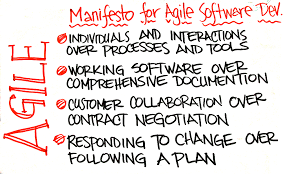
\includegraphics[width=.6\textwidth]{img/agile}
	\caption{Manifesto for Agile Software Dev.[www.medium.com]}.\label{rys:agile}% Źródło rysunku i etykieta przez którą odwołujemy się do rysunku.
\end{figure}

\newpage

Ten Manifest pokazywał pewien system wartości, co jest ważniejsze, a co mniej ważne w zarządzaniu projektem. Mamy więc takie cztery porównania:

\begin{itemize}
	\item Autorzy Manifestu twierdzili, że ludzie i interakcje między nimi są ważniejsi, niż procesy i narzędzia- to nie znaczy, że procesy i narzędzia nie są istotne, ale są mniej istotne, mniej ważne. Trzeba położyć większy nacisk na ludzi, na interakcje- to powoduje bardziej nieformalną komunikację, jej przyspieszenie, również przyspieszenie realizowania zadań i umożliwia bardziej elastyczne realizowanie tych zadań, kiedy zmieniają się warunki;
	\item Druga zasadą jest orientacja bardziej na działające oprogramowanie, niż na dokumentację. Jeśli zerkniemy do starych wersji oprogramowania z lat 80-tych, 90-tych, do każdego programu dodawana była gruba instrukcja. Dzisiaj już o tym zapomnieliśmy. Dzisiaj wiele aplikacji nie ma w ogóle nawet instrukcji- mówimy, że działają intuicyjnie (przynajmniej powinny). Dzięki temu, że orientujemy się na realizację tych najważniejszych efektów w projekcie, możemy lepiej wykorzystać zasoby, możemy szybciej osiągnąć te efekty, a rzeczy mniej ważne, mniej istotne, takie właśnie, jak szczegółowa dokumentacja (jakaś dokumentacja przecież musi być), możemy odłożyć, możemy przeznaczyć dla nich mniejsze zasoby.
	\item Również jeśli chodzi o współpracę z klientem, w metodykach zwinnych proponuje się zmianę podejścia. Zamiast negocjować szczegółowo umowy, budujemy współpracę z tym klientem dlatego, że nie jesteśmy w stanie z góry przewidzieć, jaki będzie, tak do końca, zakres naszego projektu, co w tym projekcie zrealizujemy, co będzie potrzebne za rok, kiedy nasz produkt będzie prawie gotowy. Czy te wymagania się nie zmienią wielokrotnie, biorąc pod uwagę szybkość zmiany technologii, potrzeb, oczekiwań klientów, szybkość zmian na rynku. Zatem klient powinien być blisko, powinien dostarczać bieżące informacje o swoich potrzebach, a w kontrakcie zawieramy tylko te informacje, które są najważniejsze.
	\item I w końcu reagowanie na zmiany zamiast szczegółowego planowania.
	Oczywiście planowanie występuje w metodykach zwinnych, ale jest ono ograniczone tylko do tego, żeby dało się zarządzać takim projektem. Natomiast przede wszystkim orientujemy się na reagowanie na zmiany: zmiany potrzeb klienta, zmiany na rynku. Na dostosowanie naszego projektu, w kolejnych iteracjach, do tego, czego klient oczekuje.
\end{itemize}

Czasem niektórzy mówią, może żartobliwie, ale nieraz całkiem serio, że jeżeli czegoś nie zaplanowali, to stosowali właśnie Agile. Nic bardziej błędnego: w Agile każda iteracja jest planowana, w każdym dniu planujemy swoją pracę, stosujemy inne metody, rzadko stosujemy harmonogram Gantta, ale także planujemy te działania. Zatem taki polski Agile („polnische Agile”, jak niektórzy mówią), to przykład niewłaściwego zarządzania przedsięwzięciami i raczej nie należy się tym chwalić.
Warto jednak zauważyć, że nie do każdego projektu możemy zastosować metodyki zwinne. One się lepiej sprawdzają wtedy, kiedy mamy:
\begin{itemize}
	\item bardzo krótkie, napięte terminy;
	\item projekty mają charakter unikatowy;
	\item są skomplikowane.
\end{itemize}

Mamy do zrealizowania coś nowego, nieoczekiwanego i mało czasu. Wtedy ta metodyka zwinna rzeczywiście jest bardziej uzasadniona niż metodyki klasyczne. Stosowanie metodyk zwinnych, szczególnie żądanie tej interakcji między pracownikami ogranicza nam wielkość zespołu, a więc ogranicza nam wielkość projektu. Generalnie metodyki zwinne stosujemy:
\begin{itemize}
	\item w małych i średnich projektach, rzadziej w projektach dużych;
	\item konieczne jest, aby w metodyce zwinnej dostępny był dla nas klient, klient musi się na bieżąco kontaktować z nami i mówić czego potrzebuje, jakie są jego oczekiwania, czy jest zadowolony z tego, co uzyskuje w poszczególnych iteracjach;

	\item tematyka projektu musi być taka, aby klient z każdej iteracji miał jakąś wartość, bowiem staramy się często wypuszczać oprogramowanie, często wprowadzać nowe jego wersje, ale to powoduje, że ta nowa wersja musi dostarczyć jakąś wartość dla klienta.
\end{itemize}
W przypadku oprogramowania jest to oczywiste. W przypadku, kiedy budujemy jakiś budynek, być może Agile wtedy nie jest aż tak przydatny. Trzeba się zastanowić, czy możemy zastosować całą metodykę Agile, czy jak współcześnie w wielu projektach, zastosować ją tylko w odniesieniu do wybranych modułów projektu, tam, gdzie rzeczywiście ma ona zastosowanie.

Więcej informacji można znaleźć w:\cite{Cohen_2006}

% !TeX program = latexmk
% !TeX spellcheck = pl_PL
% !TeX root = example.tex

\chapter{Najczęściej wykorzystywane narzędzia w zarządzaniu projektami}

Zarządzanie projektami informatycznymi ściśle wiąże się z wykorzystaniem narzędzi informatycznych,
które wspomagają ten proces. Przy ich wyborze warto pamiętać, iż mają pomagać w pracy projektowej,
a nie przeszkadzać w jej realizacji, dlatego należy wybierać je mądrze.
Przykładem nieodpowiedniego doboru narzędzia może być sytuacja,
w której kierownik projektu nie dotrzymuje terminów swoich prac,
ze względu na zajmowanie się raportowaniem postępu prac lub aktualizacją harmonogramu.
\cite{Kopczewski_2015}

\section{Narzędzia wspomagające podejście klasyczne}

\subsection{Microsoft Project}

Najbardziej popularnym narzędziem stosowanym w metodykach klasycznych jest Microsoft Project (\ref{rys:project}).
Pozwala on na rozpisanie całego harmonogramu działań, zaplanowanie budżetu czy stworzenie wykresu Gantta,
tak niezbędnego w pracy kierownika. Pozwala także na tworzenie raportów, prezentacji i wykresów z postępów prac.

\begin{figure}[H]
	\centering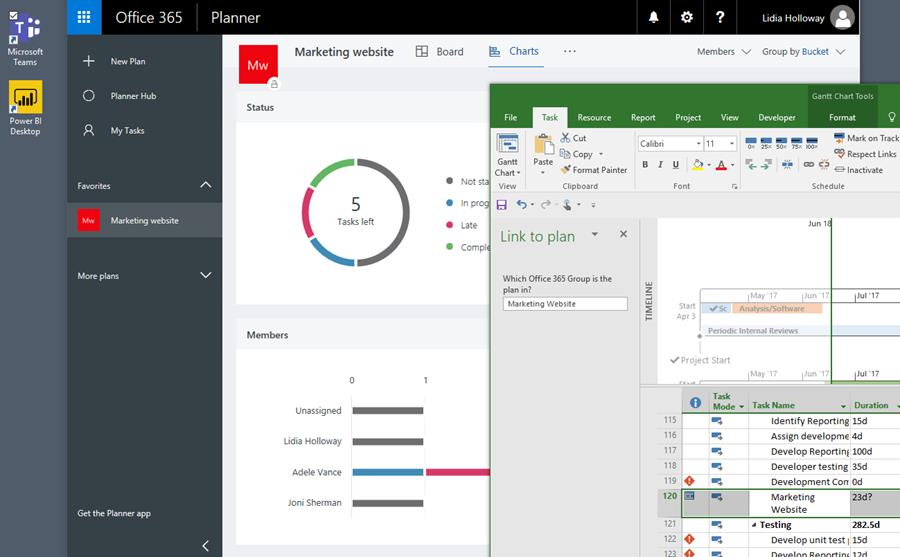
\includegraphics[width=.8\textwidth]{img/Microsoft_Project}
	\caption{Microsoft Project[www.microsoft.com]}\label{rys:project}% Źródło rysunku i etykieta przez którą odwołujemy się do rysunku.
\end{figure}

\subsection{Gantt Project}

W niektórych przedsiębiorstwach w zarządzaniu projektami używa się programu GanttProject.
Jest to darmowe narzędzie umożliwiające dynamiczne tworzenie diagramów Gantta
z podziałem na poszczególne zadania wraz z rozplanowaniem ich w czasie.
Dodatkowo pozwala ono na tworzenie wykresów PERT (ang. Program Evaluation and Review Technique)
wraz ze ścieżkami krytycznymi.
\cite{Trendy_Zarzadzanie}


\section{Narzędzia stosowane w metodykach zwinnych}

W małych zespołach projektowych, które wykorzystują metodyki zwinne,
odchodzi się zazwyczaj od Microsoft Project czy GanttProject stosując aplikacje webowe.
Przykładem takich aplikacji są: Jira, Mantis, TFS, Trello, Redmine, Kanban Tool.

Przy metodykach zwinnych, właściciel produktu tworzy rejestr produktowy (ang. Product Backlog),
który ma formę listy zawierającej wymagania klienta z określoną wagą (priorytetem) i czasochłonnością.
\cite{Shwaber_2004}

Wymienione wyżej narzędzia pozwalają na taką pracę i umieszczanie danych w chmurze,
dzięki czemu każdy członek zespołu ma do nich dostęp,
niezależnie od lokalizacji, czy pracuje w biurze czy poza nim.
Zadania w backlogu
\footnote{Backlog – rejestr sprintu / lista zadań \cite{metody_zwinne_2016}}
powinny być rozpisane dla obecnego sprintu
\footnote{Sprint – jeden z etapów niektórych metodyk zwinnych, który wyznacza rytm pracy. W jego
trakcie następuje faktyczne wykonanie określonej funkcjonalności \cite{Samoorganizacja_2010}}
oraz zawierać dodatkowe zadania, które będą zasilać kolejny sprint bądź zostaną wykonane w istniejącym,
gdy nadarzy się taka możliwość.

Takie podejście do pracy umożliwia wykonanie części zadań przed wyznaczonym czasem.
Narzędzia te pozwalają również na przypisanie konkretnego zadania do danego użytkownika,
dzięki czemu każdy pracownik zna zakres swojej odpowiedzialności.
Zapobiega to przypadkowemu wykonaniu tego samego zadania przez kilka osób.

Niektóre firmy, a można nawet powiedzieć, że wiele firm,
niezależnie od wykorzystywanej metodyki używa narzędzie Microsoft Excel do zarządzania projektami.
Umożliwia ono przedstawienie danych w postaci tabeli oraz różnych grafów.
Każda firma może zarządzać nim na swój własny sposób, dzięki czemu proces ten jest bardzo elastyczny.
Ponadto ułatwia on wykonanie prognoz przyszłych dochodów, kalkulacji wybranych parametrów i wskaźników.

Kolejnym narzędziem wykorzystywanym na szeroką skalę jest SharePoint,
który umożliwia współdzielenie plików czy tworzenie listy zadań,
która może być wykorzystana w MS Project.

\section{Narzędzia wspomagające proces estymacji zadań projektowych}

W klasycznych projektach tworzymy harmonogramy, szczegółowe plany, gdzie mamy daty,
gdzie mamy godziny, gdzie każde zadanie ma określony czas realizacji.
W przypadku projektów zwinnych często odchodzimy od tak szczegółowego planowania.
ale jakaś forma planowania oczywiście jest potrzebna.
W projektach zwinnych bardzo często planujemy bez użycia dni i godzin.
Dlatego stosujemy różne alternatywne metody i jedną z takich alternatywnych metod
jest metoda zwana Team Estimation Game.

\subsection{Team Estimation Game}

Team Estimation Game działa tak:

\begin{itemize}
	\item Członkowie zespołu kolejno pobierają kartę ze stosu i przyklejają ją do ściany.
	Każda karta przedstawia jedną historyjkę.
	Po umieszczeniu pierwszej karty w środku, każdy członek zespołu umieszcza swoją kartę po prawej,
	jeśli jest trudniejsza, po lewej, jeśli jest mniej trudna,
	lub pod inną kartą, jeśli historyjki są mniej więcej takiej samej złożoności
	(patrz \ref{rys:teamEstimationGame}).
	\item Użytkownik może użyć swojej kolejki, aby przesunąć kartę już na ścianie po prawej lub lewej stronie.
	\item Proces może być kontynuowany po tym, jak stos kart zostanie zużyty,
	aż do ogólnego konsensusu w rankingu kart. Gracze mogą omawiać historie i wpływać na swoje decyzje.
	\item Następnie każdy członek drużyny odbiera kartę z numerem i umieszcza ją na jednej z kolumn.
	Członek zespołu może użyć swojej kolejki, aby zmienić przypisanie numeru
	wykonane przez innego członka zespołu. Trwa to aż do osiągnięcia konsensusu.
\end{itemize}

\begin{figure}[H]
	\centering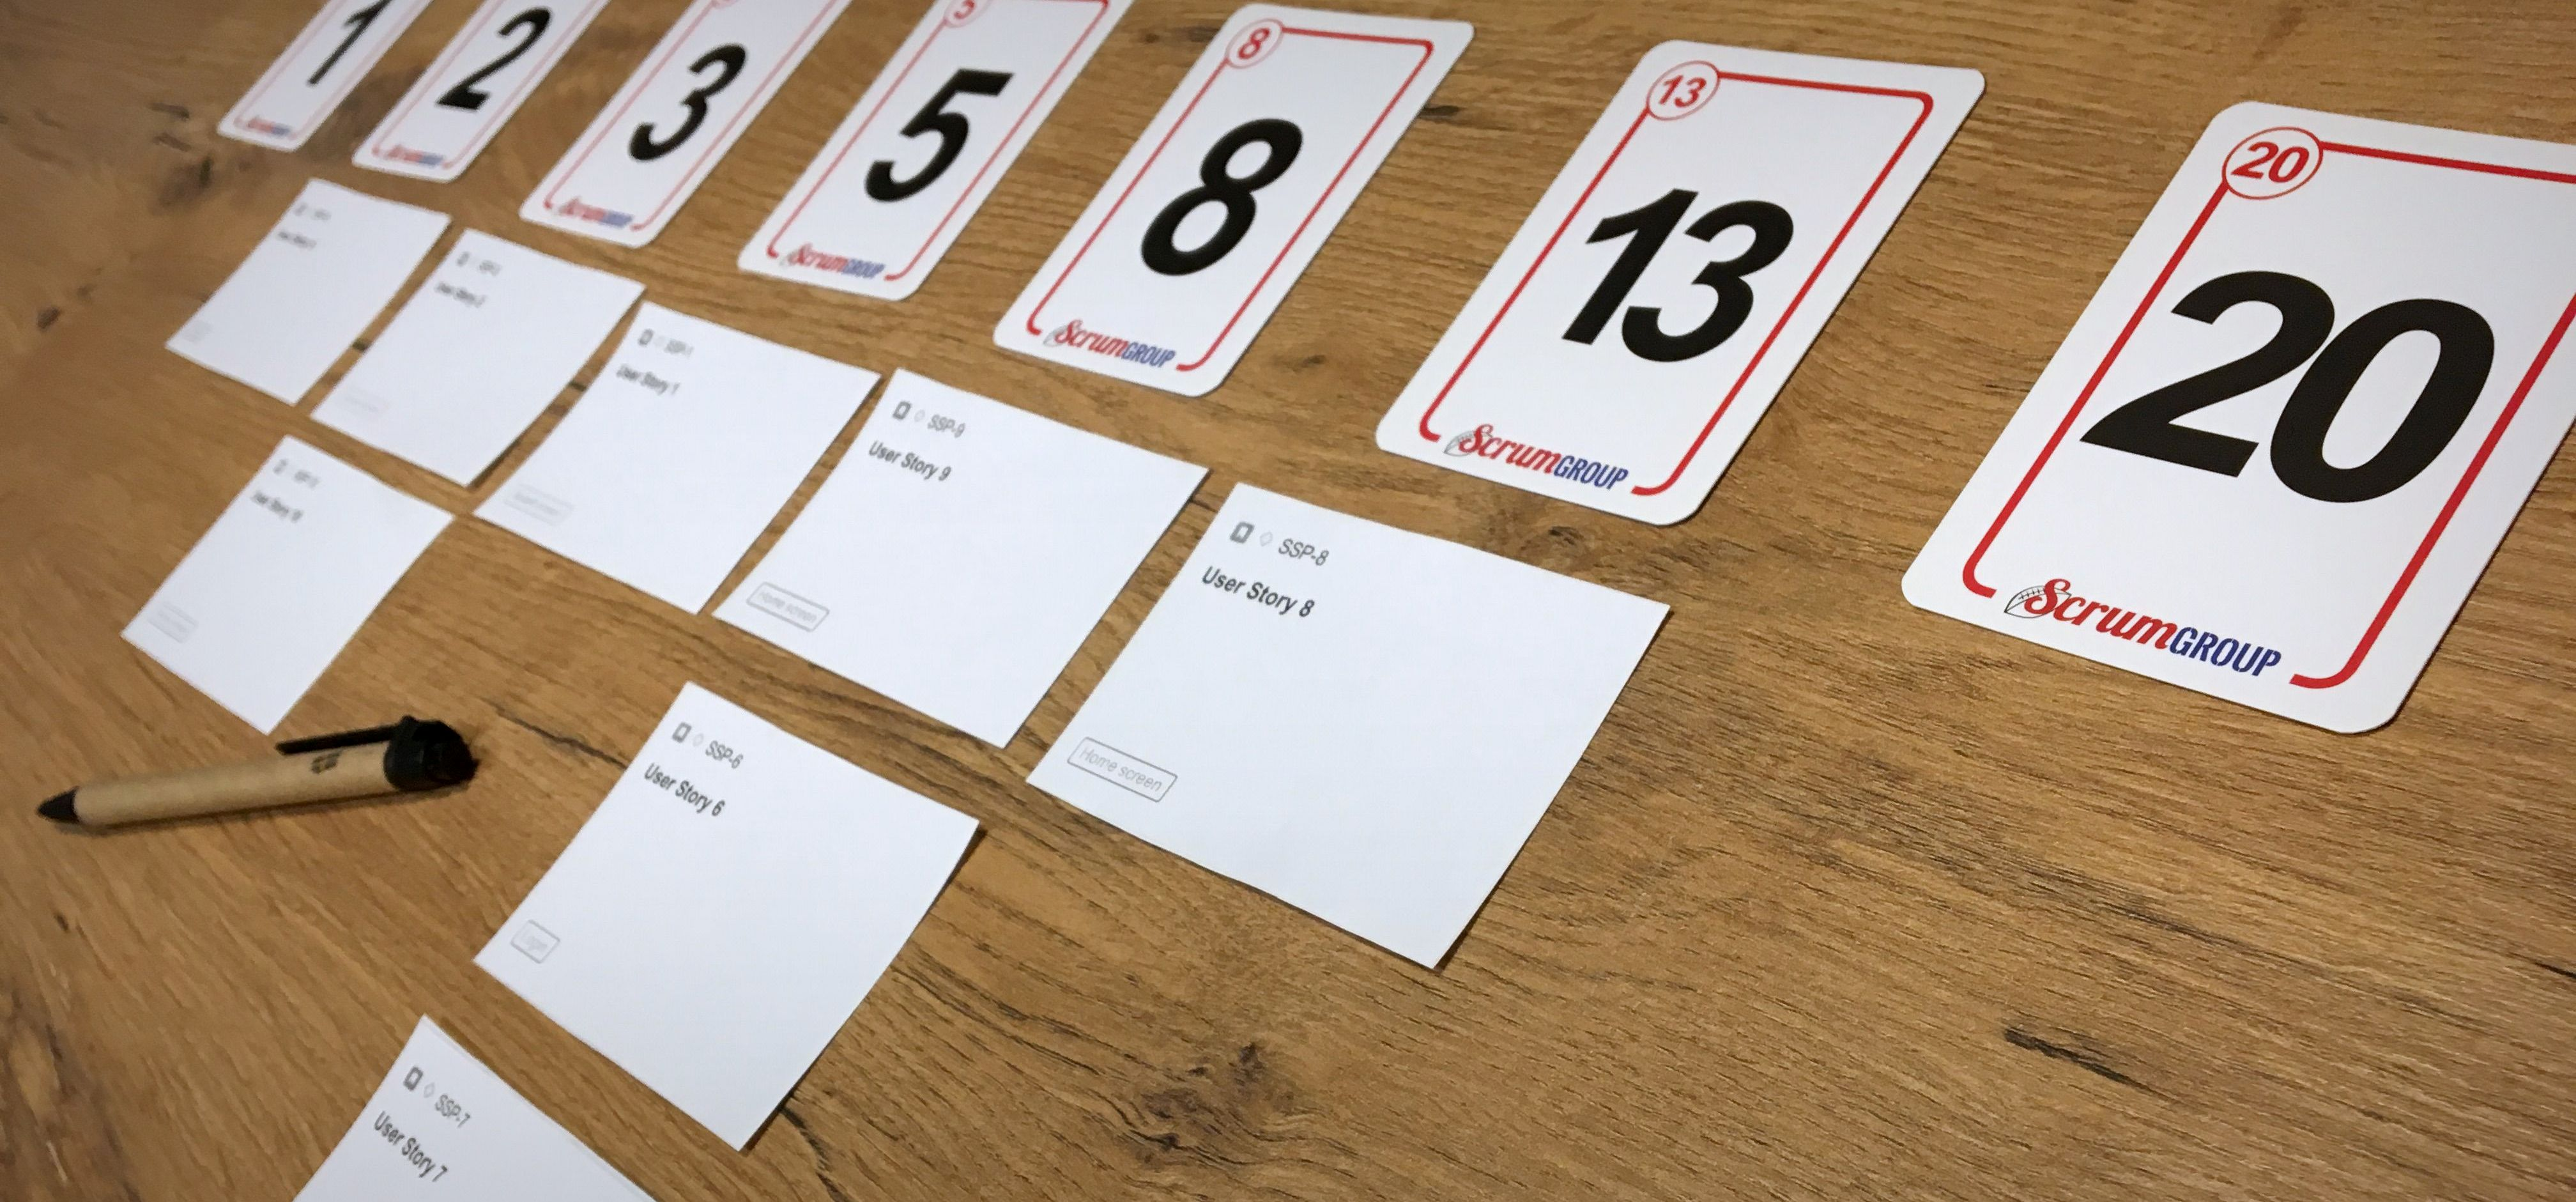
\includegraphics[width=.6\textwidth]{img/team_estimation_game}
	\caption{Team Estimation Game [www.scrum-master.pl]}
	\label{rys:teamEstimationGame}
\end{figure}

Zbiór liczb zawiera tylko te w sekwencji Fibonacciego, aby odzwierciedlić ogólną zasadę,
że ryzyko wzrasta geometrycznie proporcjonalnie do złożoności.

\subsection{Kanban}

Inną z takich alternatywnych metod jest metoda Kanban. Kanban, to koncepcja wzięta z produkcji,
która została świetnie zaadaptowana właśnie do zarządzania projektami zwinnymi.
Kanban w przypadku projektów jest po prostu tablicą, na której pokazujemy,
rejestrujemy to, co się dzieje w projekcie (patrz \ref{tabela:kanban}).

Zaczynając od lewej strony tej tablicy, mamy backlog produktu, a więc wszystkie nasze historyjki,
które określają to, co jest w projekcie do realizacji.
Następnie mamy trzy główne etapy realizacji projektu, w których nasze historyjki będą się za chwilę znajdowały:

\begin{itemize}
	\item Pierwszym takim etapem jest \textit{breakdown} albo \textit{analysis}, czyli analizowanie historyjek,
	rozbijanie ich na mniejsze części, na zadania, analiza tego co jest do zrobienia, w jaki sposób mamy te zadania zrealizować.
	W tym miejscu musimy także zastanowić się nad kompatybilnością i powiązaniami pomiędzy poszczególnymi zadaniami,
	a także nad priorytetami. Dlatego bierzemy przede wszystkim te rzeczy, które mają wysoki priorytet oraz wszystkie funkcje,
	które są z nimi powiązane, abyśmy mogli dostarczyć nowy produkt.
	\item Kolejny etap, to jest rozwój (ang. \textit{develop}) - w sytuacjach, gdzie opracowujemy nasz projekt,
	a więc tutaj zespół tworzy faktycznie te rozwiązania, które miały być opracowane.
	\item Trzeci etap, to \textit{validate}, czyli kontrola, testy, ocena tego, co zostało zrobione.
	Sprawdzamy czy rzeczywiście to, co miało być osiągnięte, zostało osiągnięte.
	Jeżeli tak, możemy dołączyć te funkcjonalności do produktu i przekazać je do klienta.
\end{itemize}

W każdym z tych etapów widzimy co najmniej dwie kolumny:

\begin{itemize}
	\item jedna kolumna, to \textit{working}, czyli pracujemy nad czymś,
	\item druga kolumna, to \textit{done}, czyli "wykonane" - wykonaliśmy to zadanie
	i dalej zadanie może przejść do kolejnego etapu, do kolejnej części prac.
	\item Dodatkowo, w przypadku kolumny związanej z rozwojem, mamy taką kolumnę \textit{track}
	– to sytuacja, w której opracowaliśmy jakąś funkcjonalność,
	ale nie jesteśmy jej w stanie wdrożyć dalej, ponieważ czekamy na opracowanie innych,
	powiązanych z nią funkcjonalności.
	Czasem jest tak, że pewna funkcjonalność może być już gotowa, ale nie może działać,
	dopóki inne elementy nie zostaną przygotowane.
	Dlatego jest takie pole oczekiwania na inne elementy, które muszą być przygotowane.
\end{itemize}

\begin{table}
	\centering\caption{Tablica w metodzie Kanban.}\label{tabela:kanban}
	\begin{tabular}{*8{l} }% wyrównanie kolumn tabeli -> l c r - do lewej, środka, do prawej
	\toprule
	\multicolumn{1}{|c|}{\textbf{Backlog}} &\multicolumn{2}{|c|}{\textbf{Breakdown (10*)}} & \multicolumn{3}{|c|}{\textbf{Develop (15*)}} & \multicolumn{2}{|c|}{\textbf{Validate (10*)}} \\
	\midrule
	Epics,User Stories & Working
	& Done & Working & Track & Done & Working & Done \\
	\bottomrule
	\end{tabular}
\end{table}

Widzimy więc, że w tej metodyce nie mamy iteracji jako takich, mamy stały przepływ historyjek,
stały przepływ pracy, która jest realizowana w naszym projekcie.
Ale ktoś może zapytać, w jaki sposób razie określamy poziom wykonania prac, w jaki sposób określamy
ile tej pracy możemy mieć jednocześnie rozpoczętej?
Temu służą te liczby w nawiasach, które widzimy w nagłówku tabeli.
Te liczby określają nam liczbę punktów, które mogą być aktualnie w obróbce.

Historyjki oceniamy nie względem czasu, lecz względem punktów trudności,
punktów zaangażowania, które jest niezbędne, aby daną funkcję zrealizować.
Jeżeli zatem w danym etapie naszej tablicy Kanban mamy dopuszczone 10 punktów,
to znaczy, że możemy tam mieć w trakcie obróbki historyjki,
których suma punktów estymacji nie przekracza 10-ciu. Tak samo w kolejnych etapach.
Zatem to określa nam poziom pracy, która jest wykonywana i powoduje, że praca będzie przebiegać płynnie,
nie będzie korków, nie będzie zatrzymań i będziemy w stanie w odpowiednim czasie dostarczać klientowi
nowe produkty.

\subsection{Planning Poker}

Jeszcze inną z takich alternatywnych metod (bardzo popularną) jest metoda,
której poświęcona jest niniejsza praca.
Ta metoda nazywa się \textit{Planning Poker} i pozwala nam oszacować trudność,
czasochłonność poszczególnych zadań, które są do wykonania w ramach projektu.
Ta metoda ma też tą zaletę, że integruje zespół i pozwala uwzględnić różne punkty widzenia,
a także przyczynia się do lepszego zrozumienia zadań, które są do wykonania.
O co w tej grze chodzi? Bazujemy tutaj z grubsza na liczbach z ciągu Fibonacciego (patrz \ref{rysunek:poker}).

Określamy trudność poszczególnych zadań wykorzystując kolejne liczby z tego ciągu: 1, 2, 3, 5, 8,13, 21 itd.
Jeżeli jakieś zadanie oceniliśmy na 5, to znaczy, że jest ono trudniejsze od zadania, które oceniliśmy na 3,
ale ile ono zajmie? Tego nie wiemy, to nas chwilowo nie interesuje.
Staramy się określić, przede wszystkim, na ile trudne i na ile pracochłonne, naszym zdaniem, mogą być zadania.

Praktyka pokazuje, że planując sprinty, wcale nie musimy mieć szczegółowych informacji na temat czasu,
te informacje zresztą często się nie sprawdzają.
Taka forma punktowa zupełnie nam wystarcza. Kiedy wiemy, ile jesteśmy w stanie w ciągu sprintu
zrealizować takich punktów, to wówczas jesteśmy w stanie stwierdzić, ile możemy zadań w danym sprincie upchnąć.

Rozgrywka Planning Poker odbywa się następująco:

\begin{itemize}
	\item Zespół programistów spotyka się na spotkaniu, siada przy stole,
	każdy otrzymuje swoje karty i mamy pakiet zadań (czy pakiet historyjek) z backlogu,
	którymi się musimy zająć.
	Zazwyczaj spotkanie prowadzi scrum master lub właściciel produktu (ang. Product Owner),
	przedstawia on historyjkę, którą mamy się zająć, określa czego ona dotyczy.
	\item Następnie każdy z członków zespołu wyciąga kartę, która jego zdaniem dobrze określa trudność,
	realizacji tego zadania i kładzie ją na stole tak, aby nie było widać tej liczby.
	\item Kiedy wszyscy są gotowi, odwracamy karty i patrzymy czy wynik, który uzyskaliśmy jest zgodny,
	czy też nie. Jeżeli wszyscy pokazali praktycznie tą samą liczbę, to sprawa jest załatwiona.
	To znaczy, że wszyscy rozumiemy zadanie w taki sam sposób, tak samo oceniamy jego trudność
	i możemy przejść do kolejnego.
	\item Kiedy jednak występuje zróżnicowanie, konieczna jest dyskusja.
	Pytamy osoby, która podała najniższą liczbę, dlaczego tak uważa.
	Pytamy osoby, która podała najwyższą liczbę, dlaczego tak uważa.
	Bardzo często te różnice wynikają z tego, że nie do końca rozumiemy zadanie.
	Po dyskusji, gdy żaden z członków zespołu nie ma już wątpliwości co do
	szczegółów omawianego zadania, można powtórzyć rozgrywkę, która zazwyczaj dzięki
	odbytej dyskusji, kończy się konsensusem.
\end{itemize}

\begin{figure}[H]
	\centering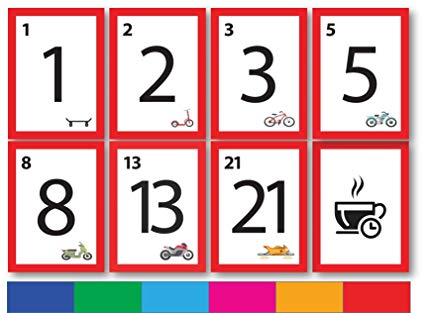
\includegraphics[width=.6\textwidth]{img/Planning_Poker}
	\caption{Przykładowe karty do Planning Pokera}\label{rysunek:poker}
\end{figure}

A więc Planning Poker pozwala nam lepiej zrozumieć zadania w zespole,
dzięki czemu nie ma później nieporozumień i dzięki czemu to planowanie jest bardziej precyzyjne.
Kiedy przejdziemy przez wszystkie historyjki i odzwierciedlimy, oszacujemy ich trudność w punktach,
możemy przejść do planowania sprintu.

Z doświadczenia wiemy, że nasz zespół jest w stanie zrealizować określoną liczbę punktów w ciągu danego sprintu.
Ta liczba nazywa się \textit{team velocity}, czyli szybkość, z jaką zespół pracuje.
Jest typowa dla każdego zespołu, a więc nie jest tak, że jeżeli jeden zespół
jest w stanie zrealizować 30 punktów, to każdy inny będzie w stanie tyle samo zrealizować.

Co więcej, nie można tej liczby traktować jako wskaźnika motywacji
(zróbcie pięć punktów więcej, to dostaniecie premię) dlatego,
że zaobserwowano, iż w takich przypadkach każde kolejne szacowanie po prostu powoduje,
że członkowie zespołu przydzielają więcej punktów, czyli określają zadania jako trudniejsze,
niż są w rzeczywistości, a więc mamy taką inflację punktów - nie ma realnego
zwiększenia realnego wykonanej pracy, jest po prostu zwiększenie liczby punktów.
Taki sposób motywacji nie jest zatem dobrym pomysłem.

Dzięki tej metodzie możemy odejść od określania, czy coś będzie trwało 2,5 godziny,
czy 3,5 godziny, możemy skupić się na lepszym zrozumieniu zadań,
jak również na tym, aby lepiej rozplanować pracę.


% !TeX program = latexmk
% !TeX spellcheck = pl_PL
% !TeX root = example.tex

\chapter{Rozproszone zespoły projektowe.}

Według niemieckiego pisma Focus Money Magazin, ok 30 \% wszystkich pracowników na świecie (a podobno w USA ponad 43 \%) pracuje w tzw. zespołach rozproszonych lub wirtualnych. Wiele firm wprowadza zarządzanie na odległość, aby w ten sposób stymulować rozwój, rozwijać projekty międzynarodowe, czy chociażby ze względu na oszczędności lub optymalizację procesów.

Pojawienie się zjawiska zespołów rozproszonych może się wiązać z efektem globalizacji obszaru działania firm, wkraczaniem na nowe rynki, powstawaniem startupów, jak również działaniem tzw. freelancerów, którzy oferują wyspecjalizowane usługi. Powodem może być również wzrost kosztów pracy, zmiany na rynku pracy oraz brak na rynku lokalnym wykwalifikowanych pracowników, jak i również zmiany w kulturze pracy (np. pokolenie tzw. Milenialsów). Wszystko to powoduje zmiany w organizacji pracy.

\section{Zalety zarządzania projektami w zespołach rozproszonych.}

Realizacja projektów zespołami rozproszonymi:

\begin{itemize}
	\item pozwala na pozyskiwanie profesjonalistów w ramach całej organizacji lub poza nią;
	\item niweluje problem ograniczeń korzystania wyłącznie z zasobów jednego biura, czy w ramach jednego kraju;
	\item daje szerokie możliwości czerpania z dużo większych zbiorów doświadczeń oraz kreatywności;
	\item pozwala na elastyczność w rozbudowywaniu zespołu adekwatnie do pojawiających się nowych zadań;
	\item daje organizacjom szansę dostosowywania się do zmian pokoleniowych, gdzie często młode osoby wyrażają potrzebę wykonywania pracy w domu (Home Office);
	\item zwiększa efektywność kosztową.
\end{itemize}

\section{Dodatkowe wyzwania dla efektywnego funkcjonowania zespołów rozproszonych.}

Każdy zespół projektowy napotyka w swojej pracy na najróżniejsze wyzwania, które związane są ze współpracą, komunikacją, czasami niejasnym podziałem obowiązków, brakiem odpowiedzialności, czy zaangażowaniem. Jednak zespoły rozproszone stają często przed dodatkowymi wyzwaniami, jakie wynikają z ich specyfiki, czyli pracy w różnych lokalizacjach.

Oto kilka najczęstszych wyzwań takich zespołów:

\begin{itemize}
	\item \textbf{Zarzadzanie zespołem i synchronizacja pracy jego członków.}
	To wyzwanie nie tylko dotyczy zespołów rozproszonych, ale w właśnie w takich zespołach ważna jest umiejętność prowadzenia projektu i kwalifikacje związane z zarządzaniem ludźmi. W zespole rozproszonym powinny funkcjonować jasne zasady współpracy i komunikacji. Bardzo istotne jest ogólne zaangażowanie, wzajemne rozliczanie się z zadań, odpowiedzialność za rezultaty, otwartość, szacunek dla innych, zakładanie zawsze dobrych intencji, jasny podział obowiązków. Ważne jest również dla budowania zespołu i jego efektywności, aby zaplanować (w budżecie oraz czasowo) okresowych, wspólnych spotkań wszystkich członków.
	\item \textbf{Przepływ informacji.}
	Czasem kluczowe informacje nie docierają do wszystkich członków zespołu. Odpowiedzią na to może być ustalenie pewnego „rytmu” komunikacyjnego i regularne spotkania projektowe. Muszą to jednak być spotkania z sensem, tak zaplanowane, aby nie marnować czasu pracowników, aby rozwiązywały konkretne problemy i wspierały realizację celów projektu. Sposobów komunikacji jest wiele, można zatem je dobrze zaplanować i stosować w zależności od złożoności zespołu, celu i rodzaju projektu.
	\item \textbf{Komunikacja w obcym języku.}
	Coraz powszechniejsza jest konieczność porozumiewania się w języku obcym, ponieważ wiele firm posiada zagraniczne filie i siedziby. Zazwyczaj wykorzystywany do komunikacji jest język angielski, ale poziom jego znajomości może być różny i może powodować różne zabawne sytuacje lub nawet nieporozumienia. Tutaj może pomóc np. nauka prostych technik coachingowych- pytań doprecyzowujących i tzw. uważne słuchanie.
\end{itemize}

Jednak zespoły rozproszone muszą się borykać z problemami takimi jak: Różnica czasu, Różnice kulturowe, Odpowiednia rekrutacja, Motywowanie i wsparcie zespołu, Efektywność i produktywność, zwiększa efektywność kosztową

Dochodzimy wreszcie do kwestii, które próbuję rozwiązać, realizując projekt, który jest zasadniczym tematem niniejszej pracy inżynierskiej. Jest to wyzwanie:

\begin{itemize}
	\item \textbf{Wsparcie techniczne i merytoryczne.}
	W zespołach rozproszonych wręcz niezbędne jest zadbanie o wsparcie techniczne. Co więcej, wielu menedżerów zarządzających zespołami rozproszonymi, wskazuje na potrzebę wsparcia merytorycznego , szczególnie w zakresie moderowania tzw. metodyk zwinnych (SCRUM). Świetne połączenie internetowe, sprzęt , sale i programy do tele i wideokonferencji, to powinien być standard w organizacjach, które pracują w zespołach wirualnych.
\end{itemize} 

Więcej informacji o zespołach rozproszonych można znaleźć w:\cite{www_rozproszony}

% !TeX program = latexmk
% !TeX spellcheck = pl_PL
% !TeX root = example.tex

\chapter{Implementacja projektu}

Projekt aplikacji wspomagającej zdalne szacowanie historyjek metodą planning pokera został wykonany w technologii webowej
o nazwie ReactJS oraz Firebase po stronie backendu.
ReactJS to biblioteka javascript stworzona przez firmę Facebook
oraz Instagram dzięki której budowanie dużych oraz kompleksowych interfejsów użytkownika jest łatwiejsze.
Jest ona przeznaczona do wykorzystania z innym frameworkiem, który wprowadza backend.
Podczas gdy Angular, Ember oraz Backpone są popularnymi wyborami do tego,
Firebase wprowadza najłatwiejszą i najszybszą integrację z trwałym backendem
czasu rzeczywistego do aplikacji napisanej w ReactJS – zajmuje to tylko kilka linijek w Javascript. 

\section{Czym jest ReactJS}

Twórcy ReactJS opisują go jako Widok w architekturze MVC,
nie ma na celu zastąpienie Angular’a oraz Ember’a;
zamiast tego rozszerza ich funkcjonalność przez wprowadzenie bardzo wydajnej drogi utrzymania widoku zsynchronizowanego z javascript.
Ten specjalny sos który renderuje HTML używa wyjątkowo szybkiego algorytmu wirtualnego drzewa DOM,
wprowadzający o wiele lepszą wydajność niż konkurujące platformy. Ma jednokierunkowy, reaktywny przepływ danych,
który jest znacznie bardziej zrozumiały niż tradycyjne przepływy danych.
Komponenty – podstawowe bloki aplikacji React'owych – są zorganizowane w drzewie hierarchicznym,
w którym komponenty-rodzice wysyłają dane do swoich dzieci przez zmienne właściwości.
Każdy komponent ma także zmienną stanu, która determinuje obecne dane dla tego widoku.
Za każdym razem, gdy stan jest zmieniany, komponent wywołuje metodę render, a React znajduje najbardziej efektywną metodę aktualizacji drzewa DOM\@.

Odkąd głównym zadaniem React’a jest interfejs użytkownika,
aplikacje na nim zrobione potrzebują czegoś jeszcze,
co będzie zachowywało się jak backend.
To jest miejsce gdzie wkracza Firebase.
Dodaje Model i Kontrolera w MVC do aplikacji napisanych w ReactJS, czyniąc z nich w pełni funkcjonalne aplikacje.
Używając React’owego jednokierunkowego systemu wiązania danych łatwo jest zintegrować go z Firebase.\cite{www_react}

\section{Firebase}

Firebase jest platformą dla aplikacji webowych oraz mobilnych która wprowadza
dla deweloperów mnóstwo narzędzi oraz usług by pomóc im tworzyć wysokiej jakości aplikacje oraz zwiększyć ich bazę użytkowników.

\subsection{Historia Firebase}

W 2011 roku, zanim Firebase było Firebase’em był startup nazwany Envelope.
Jako Envelope  wprowadził dla deweloperów API, które umożliwiało wprowadzenie czatu do ich strony internetowej.

Interesującym było to, że ludzie używali aplikacji by przekazywać dane, które były czymś więcej niż wiadomościami chatowymi.
Deweloperzy używali Envelope by synchronizować dane aplikacji jak stan gry w czasie rzeczywistym pomiędzy ich użytkownikami.

To doprowadziło założycieli Envelope, Jamesa Tamplina oraz Andrew Lee do pomysłu by rozdzielić chat oraz architekturę czasu rzeczywistego.
W kwietniu 2012 Firebase powstał jako oddzielna firma które wprowadziła Backend jako usługę z funkcjonalnościami czasu rzeczywistego. 

Po tym jak firma została przejęta przez Google w 2014 roku, szybko ewoluowała do wielofunkcyjnej platformy mobilnej oraz webowej jaką znamy dzisiaj.\ref{rys:firebase}

% Rysunek
\begin{figure}
\centering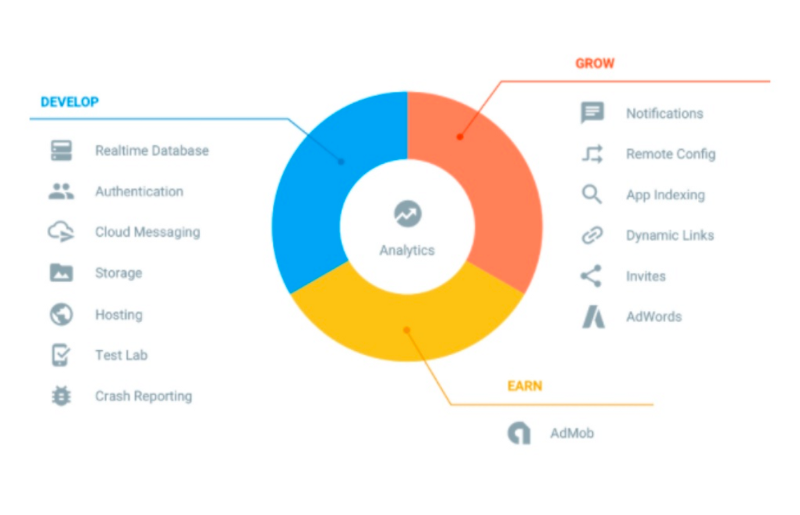
\includegraphics[width=.6\textwidth]{img/firebase}
\caption{Usługi Firebase.[hackernoon.com]}\label{rys:firebase}% Źródło rysunku i etykieta przez którą odwołujemy się do rysunku.
\end{figure}

\section{Usługi Firebase wykorzystane w pracy}

\subsection{Firebase Authentication}

W swojej aplikacji przede wszystkim skorzystałem z usługi Fierbase Authentication,
która wprowadza usługi serwerowe,
łatwe narzędzia dla deweloperów oraz gotowe biblioteki interfejsu by wprowadzić usługę logowania i rejestrowania do naszej aplikacji.

Normalnie zajęłoby miesiące by ustawić system autoryzacji na własną rękę.
A nawet wtedy twórcy musieliby mieć dedykowany zespół by utrzymywać ten system.
Ale jeżeli wykorzystają Firebase’a, mogą ustawić cały system w mniej niż 10 linijek kodu,
które zajmą się wszystkim włącznie z kompleksowymi operacjami jak scalanie kont.

Autor skorzystał z usług logowania anonimowego oraz przez Github’a co było kluczowe w projekcie.

\subsection{Firestore}

Firestore jest nierelacyjną bazą dokumentów, która pozwala łatwo przechowywać,
synchronizować oraz przeszukiwać dane dla aplikacji mobilnych oraz webowych – w globalnej skali.

Firestore przechowuje dane w postaci obiektów zwanych dokumentami.
Te dokumenty posiadają pary klucz-wartosć oraz mogą zawierać jakiekolwiek rodzaje danych od łańcuchów po dane binarne a nawet obiekty,
które przypominają drzewa JSON\@. Dokumenty są pogrupowane w kolekcje.\ref{rys:firestoreData}

\begin{figure}
	\centering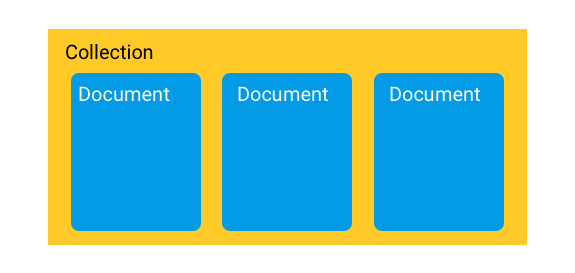
\includegraphics[width=.6\textwidth]{img/firestoreData}
	\caption{Postać danych w firestore [hackernoon.com]}\label{rys:firestoreData}% Źródło rysunku i etykieta przez którą odwołujemy się do rysunku.
\end{figure}

Fierstore może zawierać wiele kolekcji zawierających dokumenty, które wskazują na subkolekcje.
Te subkolekcje mogą znowu zawierać dokumenty oraz subkolekcje i tak dalej.
Można zatem powiedzieć że w tym modelu danych wszystko jest ułożone hierarchicznie.\cite{www_hakermoon}
rys.\ref{rys:firestoreTree}

\begin{figure}
	\centering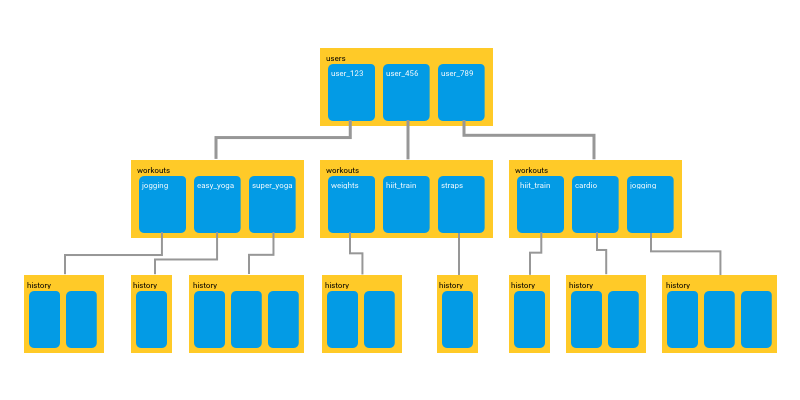
\includegraphics[width=.6\textwidth]{img/firestoreTree}
	\caption{Ułożenie danych w firestore [hackernoon.com]}\label{rys:firestoreTree}% Źródło rysunku i etykieta przez którą odwołujemy się do rysunku.
\end{figure}

\section{Redux czyli implementacja architektury Flux.}

Jedną z najważniejszych cech komponentów ReactJS jest wbudowany w nie stan.
Jest to bardzo przydatna koncepcja. Komponent posiada stan,
który może ulec zmianie w wyniku interakcji użytkownika z aplikacją.
Zmiana stanu pociąga za sobą operację re-renderowania drzewa Virtual DOM\@.
W wyniku tego, pewne części interfejsu widocznego na ekranie ulegają zmianie.
Oczywiście wiadomym jest też, że jeden komponent może zależeć od innego komponentu.
Możemy przecież przekazywać stan komponentu rodzica do jego komponentów dzieci itd.
To wszystko działa świetnie. Niestety w miarę jak aplikacja rośnie, rozrasta się poziom skomplikowania poszczególnych komponentów.
Z tego względu programiści Facebooka odpowiedzialni za rozwój ReactJS wymyślili architekturę aplikacji, która rozwiązuje ten problem.
Architektura ta nazwa się Flux.\cite{www_nafrontendzie}

\subsection{Architektura FLUX}

Flux jest architekturą, którą Facebook używa do budowania aplikacji po stronie klienta.
Jest to uzupełnienie komponentów React’a przez wykorzystanie jednokierunkowego przepływowi danych.
To jest raczej pewien wzorzec niż framework i można z niego korzystać  bez wielu nowych linijek kodu.\ref{rys:flux}

\begin{figure}
	\centering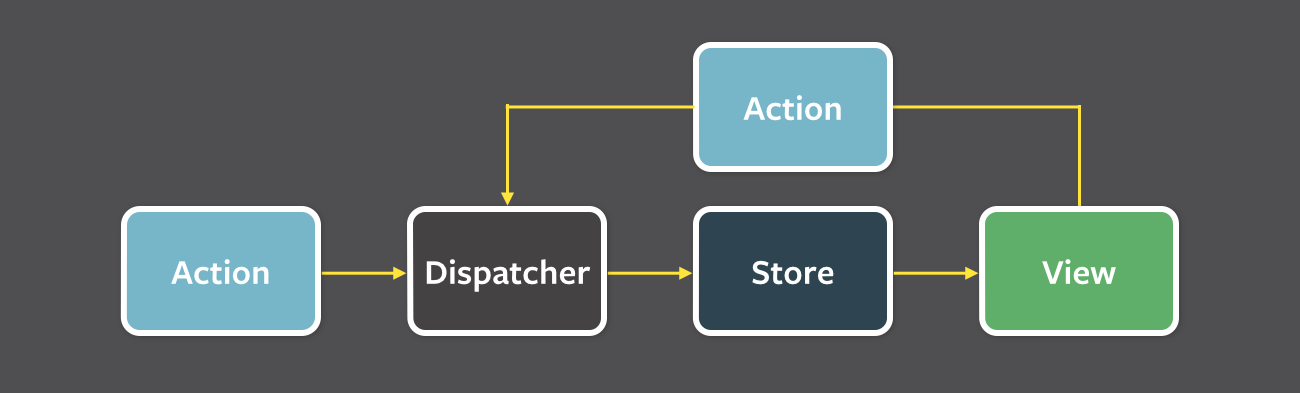
\includegraphics[width=.6\textwidth]{img/flux}
	\caption{architektura flux [wwww.nafrontendzie.pl]}\label{rys:flux}% Źródło rysunku i etykieta przez którą odwołujemy się do rysunku.
\end{figure}

Przepływ rozpoczyna się od lewej strony. Najpierw tworzone jest akcja – jest to zwykły obiekt zawierający właściwość type.
Oprócz tego może on posiadać więcej właściwości służących do przekazywania dodatkowych danych.
Akcja taka tworzona jest przez funkcję zwaną action creator czyli kreator akcji.
W przypadku redux'a jednak, akcja jest zwykłą funkcją.\ref{listing:licznik}

% lub {java} albo {bash} albo {text}
\begin{listing}
\begin{minted}{c}
const mapStateToProps = (state) => {
return { counter: state.counter };
};
const mapDispatchToProps = (dispatch) => {
return {
onIncrement: () => dispatch({ type: 'INCREMENT' }),
onDecrement: () => dispatch({ type: 'DECREMENT' })
}
};

Counter = connect(mapStateToProps, mapDispatchToProps)(Counter);
\end{minted}
\caption{Przykładowe akcje licznika i ich stan} \label{listing:licznik}
\end{listing}

W tym przykładzie przedstawiony jest prostylicznik z dwoma akcjami,
które albo zwiększają, albo zmniejszają licznik o jeden.
Stan oraz funkcję rozsyłające dostępne są w obiekcie this.props. Spójrzmy na kod odpowiedzialny za ich mapowanie.
\begin{center}
	\textbf{Funkcja mapStateToProps}
\end{center}
Funkcja \textit{mapStateToProps} pobiera \textit{state} jako parametr i zwraca nowy obiekt.
Częstą praktyką jest po prostu przekazanie całego stanu do właściwości, jednak jest to też właściwe miejsce by odfiltrować dane. 
\begin{center}
	\textbf{Funkcja mapDispatchToProps}
\end{center}
Kolejna funkcja to \textbf{mapDispatchToProps}. Zwraca ona obiekt zawierający metody.
Za pomocą wywołania funkcji \textbf{dispatch} rozgłasza ona obiekty akcji do \textbf{store}.
Metoda dispatch przekazuje obiekty akcji bezpośrednio.
Zwykle w projekcie definiuje się to jako specjalne kreatory akcji. Dzięki kreatorom możemy opóźnić wywołanie akcji,
lub zmienić dane w naszym redux'ie tylko wtedy, gdy są spełnione określone warunki. Listing 
~\ref{listing:firebase_action}

% lub {java} albo {bash} albo {text}
\begin{listing}
	\begin{minted}{c}
	export const startAddUserToGame = (owner, repo, game, user = {}) => {
	return dispatch => {
	var userUpdate = {}
	const tempUser = {
	email: user.email,
	isAnonymous: user.isAnonymous,
	id: user.uid,
	name: user.displayName,
	online: true
	};
	userUpdate[`users.` + user.uid.toString()] = tempUser
	const gameRef = db
	.collection(`users`)
	.doc(owner.toString())
	.collection(`repos`)
	.doc(repo.toString())
	.collection(`games`)
	.doc(game.toString())
	
	gameRef.update(userUpdate).then(() => {
	dispatch(addUserToGame(owner, repo, game, tempUser))
	});
	}
	}
	\end{minted}
	\caption{Przykładowy kreator akcji z projektu} \label{listing:firebase_action}
\end{listing}

W tym przykładzie gracz jest dodawany do gry tylko wtedy,
kiedy jest dodany do gry w bazie danych Firestore.
Jak widać w przykładzie kreator zwraca funkcję,
która wykorzystuje dispatch by wysłać akcję do store.
Aby zadziałać funkcja musi znać dokładną lokalizację gry w bazie oraz dane użytkownika.
Aby dostać się do gry, musimy znać właściciela oraz nazwę repozytorium w której znajduje się gra,
a później identyfikator gry.
Dzięki funkcji update gracz jest dodawany do gry dostając się odpowiednio do obiektu users,
dokumentu gry, kolekcji repozytoria, dokumentu naszego repozytorium.
Kolekcja gier znajduje się w repozytorium, a dzięki znajomości identyfikatora gry dostajemy się do jej obiektu i wstawiamy do niej obiekt gracza.
Jeżeli akcja w bazie danych zakończy się sukcesem rozsyłamy akcję dodawania gracza do store.
\begin{center}
	\textbf{Funkcja connect}
\end{center}
Wracając do mapowania. W przedstawionym wcześniej przykładzie najbardziej istotna jest ostatnia jego linia.
Wywołuję ona funkcję connect.
Przyjmuje ona funkcje mapStateToProps oraz mapDispatchToProps jako parametry i wyniki ich wywołania łączy w odpowiedni obiekt.
Następnie zwraca funkcję, która jako parametr przyjmuje komponent. Funkcja ta wprowadza przygotowany wcześniej obiekt do this.props tego komponentu.

Funkcja connect opakowuje przekazany komponent i zwraca nową jego wersję.

Wracając do FLUX.\@ Tak tworzona akcja jest dostarczana do store za pomocą wywołania funkcji zwaną dispatcher.
Funkcja ta w zasadzie zarządza całym przepływem danych.
Każdy store w aplikacji rejestruje w dispatcherze swoje funkcje wywołania zwrotnego w celu obsługi przychodzących akcji.
W momencie gdy akcja jest rozsyłana (ang dispatch), wywoływane są po kolei wszystkie te callbacki.
Jeden z nich powinien umieć rozpoznać akcję po jej typie i być przygotowany na jej odpowiednią obsługę.

\begin{center}
	\textbf{Funkcja reducer}
\end{center}

W przypadku redux'a role store'a pełni funkcja \textbf{reducer}. Dzięki temu, że jest to funkcja,
można ją jednocześnie użyć jako funkcję wywołania zwrotnego,
którą store uruchomi w momencie gdy zostanie rozgłoszona jakaś akcja.
Funkcja ta przyjmuje dwa parametry: \textbf{state} oraz \textbf{action}

Generalnie działa to tak: ktoś wywołuje akcję, obiekt \textbf{store} wywołuje funkcję \textbf{reducer},
przekazując do niej aktualny stan oraz akcję, funkcja \textbf{reducer}
sprawdza typ przekazanej do niej akcji i w zależności jak jest ten typ, zwraca nową wersję obiektu stanu.
Przykład: Listing
~\ref{listing:reducer} 

\begin{listing}
	\begin{minted}{c}
	const reducer = (state, action) => {
	switch (action.type) {
	case 'INCREMENT':
	return { ...state, counter: state.counter + 1 };
	case 'DECREMENT':
	return { ...state, counter: state.counter - 1 };
	default:
	return state;
	}
	};
	\end{minted}
	\caption{Przykładowy reducer licznika} \label{listing:reducer}
\end{listing}

W przykładzie, jeśli typ akcji to `INCREMENT' to zwracany jest nowy obiekt stanu, który ma zwiększoną o jeden wartość atrybutu counter.
Jeśli natomiast typ akcji to `DECREMENT' to zwracany jest nowy stan z atrybutem counter zmniejszonym o jeden.
Jeśli natomiast typ akcji jest zupełnie inny, obiekt stanu jest po prostu przekazywany dalej.

Generalnie wszystkie obiekty store zawierają łącznie cały stan aplikacji.
Store zawiera implementację funkcji wywoływania zwrotnego, która jest rejestrowana w „dispatcherze”, i która obsługuje akcję związane z danym store.
W redux'ie cały stan jest przechowywany w jednym obiekcie.

Kolejny element na diagramie to widok. Można powiedzieć, że jest on reprezentowany po prostu przez komponent ReactJS\@.
Używa on stanu aplikacji zapisanego w obiekcie store, tak jakby był on wewnętrznym stanem komponentu.
Zmiana stanu w store powoduje re-renderownie komponentu.
Dodatkowo komponent widoku może rozsyłać kolejne akcje, na przykład kiedy użytkownik kliknie na jakiś guzik na ekranie.
To powoduje zmianę stanu zapisanego w store.
W redux'ie komponent ma dostęp do akcji i stanu dzięki wspomnianej przeze mnie wcześniej funckji connect.

Wszystko to po prostu zestaw zasad.
To programista może zdecydować jak to dokładnie będzie zaimplementowane.
Na szczęście nie jest on zdany sam na siebie poniewać istnieje kilka gotowych implementacji architektury Flux w postaci bibliotek.\cite{www_nafrontendzie}
Jedną z nich jest oczywiście redux.

\subsection{Czym redux różni się od Flux}

Redux jest inspirowany pewnymi ważnymi cechami architektury Flux.
Tak jak Flux, Redux przepisuje twój model danych do oddzielnej warstwy twojej aplikacji (“stores” in Flux, “reducers” in Redux).
Tak jak we Flux wszystkie operacji na danych są opisywane w postaci akcji.
W przeciwieństwie do Flux Redux nie ma konceptu rozsyłacza,
ponieważ opiera się na czystych funkcjach zamiast emiterów akcji,
a czyste funkcje są łatwe do tworzenia i nie potrzebują żadnej encji (reprezentacja wyobrażonego lub rzeczywistego obiektu) by zarządzać nimi.
Jest to więc pewne odstępstwo od Flux’a.\cite{www_nafrontendzie} 

Inną ważną różnicą od Flux’a jest to że Redux zakłada że dane są niemutowalne.
Możesz używać używać statycznych obiektów oraz tablic dla swojego stanu,
ale mutowanie ich wewnątrz reducerów jest silnie nierekomendowane,
dlatego po zmianie stanu zawsze powinien być zwracany nowy obiekt.
Ogólnie Redux może być opisany przez trzy fundamentalne zasady:
rys.\ref{rys:reduxFlux}
\begin{itemize}
	\item Pojedyncze źródło prawdy: stan całej aplikacji przetrzymywany jest w drzewie obiektów wewnątrz pojedynczego obiektu store.
	\item Stan jest tylko do odczytu: jedynym sposobem na zmianę stanu jest wywołanie akcji, która zwraca obiekt opisujący co powinno się stać.
	\item Zmiany wykonywane są w ramach czystych funkcji: aby określić jak drzewo stanu transformowane jest przez akcje musisz tworzyć “czyste reducery”.
\end{itemize}

\begin{figure}
	\centering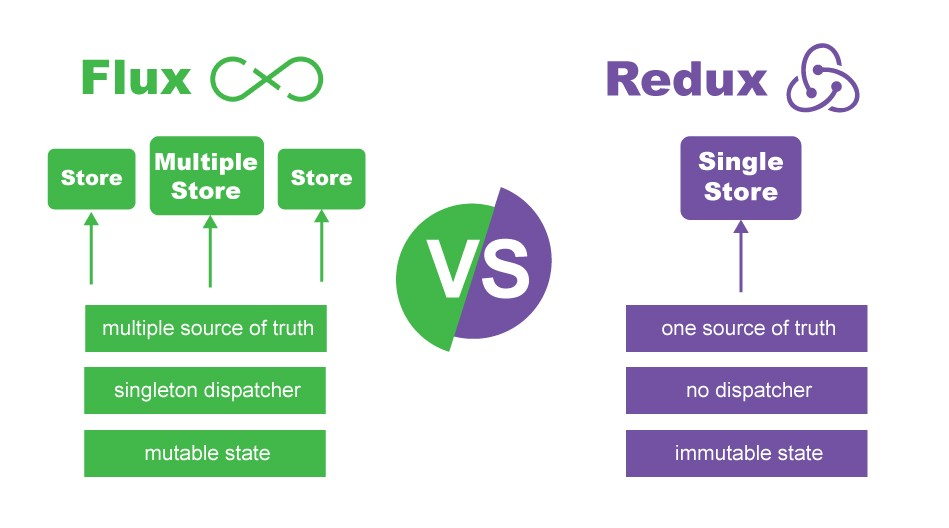
\includegraphics[width=.6\textwidth]{img/reduxFlux}
	\caption{Różnice między Redux a Flux [www.medium.com]}\label{rys:reduxFlux}% Źródło rysunku i etykieta przez którą odwołujemy się do rysunku.
\end{figure}

\subsection{redux-thunk}

Biblioteka redux-thunk została stworzona przez Dana Abramova,
który jednocześnie jest twórcą Reduxa. Pozwala ona tworzyć kreatory akcji,
które zamiast obiektu zwracają funkcję.
Dzięki temu możliwe jest opóźnienie rozgłoszenia akcji lub zgłoszenie jej tylko jeśli zostaną spełnione określone warunki.\cite{www_thunk}
Jak dodać thunk do reduxa: Listing 
~\ref{listing:thunk-redux}

\begin{listing}
	\begin{minted}{c}
	import { createStore, applyMiddleware } from 'redux';
	import thunk from 'redux-thunk';
	import rootReducer from './reducers/index';
	
	const store = createStore(
	rootReducer,
	applyMiddleware(thunk)
	);
	\end{minted}
	\caption{Połączenie Reduxa i Thunka} \label{listing:thunk-redux}
\end{listing}

\newpage

\begin{center}
	\textbf{Obsługa wywołań asynchronicznych czyli kreatory akcji}
\end{center}

W przykładzie listing 
~\ref{listing:firebase_action} widnieje akcja,
która najpierw dodaje użytkownika do bazy a później rozgłasza akcję dodawania użytkownika,
jeżeli modyfikacja danych w bazie zakończyła się pomyślnie.
W funkcji \textbf{startAddUserToGame} pobierane są najpierw dane o grze, czyli: \textbf{owner},
który jest po prostu identyfikatorem użytkownika Githuba,
który jest właścicielem repozytorium, którego nazwa jest w zmiennej \textbf{repo}.
Następnie jest pobierany identyfikatory gry (\textbf{game}).
Na końcu dostajemy dane użytkownika, którego chcemy dodać do gry.
Funkcja ta zwraca funkcję przyjmującą parametr \textbf{dispatch},
który służy do rozgłaszania danych.
Później jest tworzony użytkownik, który ma zostać dodany do gry (\textbf{tempUser}).
Na końcu jest tworzony obiekt, będący odnośnikiem do użytkowników w bazie,
który pomaga zaktualizować obiekt gry.
Następnie jest tworzona referencja do obiektu gry w bazie danych (\textbf{gameRef}).
Finalnie korzystając z referencji aktualizuje się obiekt gry w bazie danych,
 a w razie sukcesu (funkcja \textbf{then}) akcja jest rozsyłana dalej.

\subsection{Połączenie Firebase i redux’a}

Jak nie trudno się domyśleć wszystkie operacje pomiędzy Firebase a Redux są realizowane w postaci akcji.
Do synchronizacji frontend’u z backend’em służy Thunk,
który przesyła dane do store’a tylko wtedy,
kiedy nie ma żadnych problemów po stronie firebase’a.
Jeżeli baza danych nie będzie mogła pobrać danych bo wystąpił błąd,
Thunk nie wykona operacji. Sposób połączenia tych dwóch elementów przedstawiono na rys. 
~\ref{rys:fireRedux} 

\begin{figure}
	\centering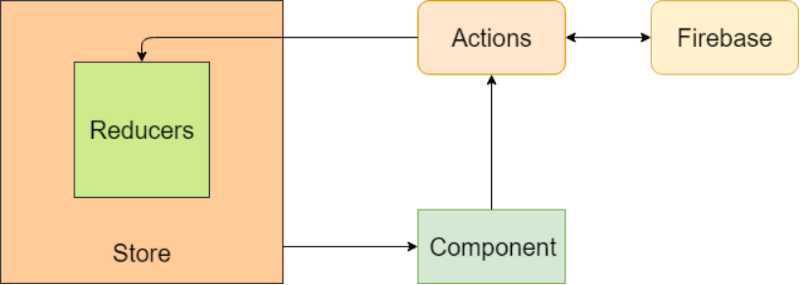
\includegraphics[width=.6\textwidth]{img/fireRedux}
	\caption{Sposób połączenia firebase i reduxa. [medium.com]}\label{rys:fireRedux}% Źródło rysunku i etykieta przez którą odwołujemy się do rysunku.
\end{figure}


\chapter{Omówienie działania aplikacji}

ĄĆĘŁŃÓŚŹŻ ąćęłńóśźż\footnote{Przykład użycia polskich znaków diakrytycznych oraz przypisu w miejscu}. \lipsum[1]

\section{Odniesienie do pozycji z literatury (strona WWW)}

% Odniesienie do rysunku i cytowanie dokumentu. Dokumenty są definiowane w pliku literatura.bib
Reszta dokumentacji znajduje się w \cite{docker_compose_reference}. \lipsum[3]

\section{Odniesienie do książki}

Jak pisze Harel w \cite{harel_rzecz_2008}: \lipsum[7]

\section{Rysunek}

% Rysunek
\begin{figure}
\centering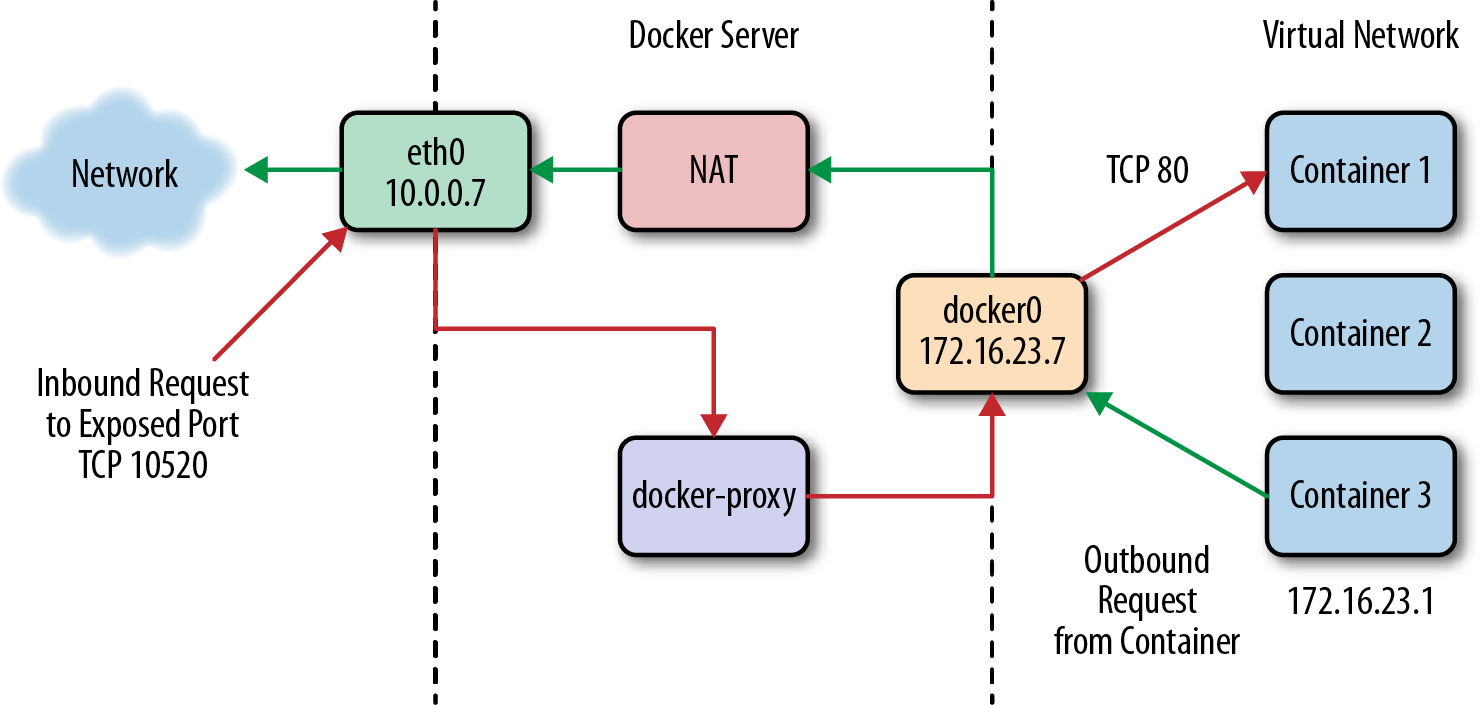
\includegraphics[width=.6\textwidth]{img/swarm-network}
\caption{Docker ma sieć \cite{docker_compose_reference}.}  \label{rys:network}% Źródło rysunku i etykieta przez którą odwołujemy się do rysunku.
\end{figure}

Jak widać na rys. \ref{rys:network} Docker ma wewnętrzną sieć. \lipsum[1]


\subsection{Rysunek z kotem}

Jak widać na rys.\ref{rysunek:kot} Ala ma kota. \lipsum[9-10] 

\begin{figure}
\centering
\includegraphics[width=.4\textwidth]{img/kotek}
\caption{Ala ma kota (opr.wł).}\label{rysunek:kot}
\end{figure}

\subsection{Tabela}

Co uwzględniono w tabeli \ref{tabela:coktoma}. \lipsum[13-15] 

% Tabela. Nazwa tabeli u góry.
\begin{table}
\centering\caption{Co kto ma \cite{harel_rzecz_2008} (patrz też dodatek~\ref{Dod1}) \label{tabela:coktoma}}
\begin{tabular}{|l|l|l|}% wyrównanie kolumn tabeli -> l c r - do lewej, środka, do prawej
\hline
Ala & ma & kota \\
\hline
Ola & ma & psa \\
\hline
Ula & ma & małpę\\
\hline
\end{tabular}
\end{table}

\lipsum[19-20] Warto wspomnieć, że w \cite{aizawa_groundwater_2009} rzecz przedstawiona jest zupełnie inaczej. Poniższy wzór:

\begin{equation}
\sum_{i=1}^{\infty}a_i
\label{eq:mojWzor}
\end{equation}

Wzór \ref{eq:mojWzor} wskazuje że dowód podany w \cite{kaleta_experimental_2005} może zostać podważony. \lipsum[9]

\section{Listing}

% lub {java} albo {bash} albo {text}
\begin{listing}
\begin{minted}{c} 
int main()
{
   int a=2*3;
   printf("**Ala ma kota\n**");
   while(!I2C_CheckEvent(I2C1, I2C_EVENT_MASTER_MODE_SELECT)); /* EV5 */
   return 0;
}
\end{minted}
\caption{Przykładowy algorytm w języku C (opr. wł.)} \label{listing:moj}
\end{listing}

W moim kodzie \ref{listing:moj} zrobiłem coś wspaniałego. \lipsum[4]


\chapter*{Zakończenie}

W pracy udało mi się dużo zrobić. \lipsum[17]

Mnóstwo innych rzeczy da się poprawić i rozwinąć. \lipsum[23]

\appendixpage
\appendix
%\addappheadtotoc

\chapter{To powinien być dodatek}\label{Dod1}


% W pracy pojawi? si? tylko prace naprawd? cytowane.
% \nocite{*}

\bibliography{literatura}
\bibliographystyle{dyplom}

\end{document}
